\documentclass[11pt,a4paper]{article}
\usepackage[utf8]{inputenc}
\usepackage[T1]{fontenc}
\usepackage[margin=2.4cm]{geometry}
\usepackage{graphicx}
\graphicspath{{../img/}}
\usepackage{booktabs}
\usepackage{longtable}
\usepackage{array}
\usepackage{xcolor}
\usepackage{enumitem}
\usepackage{float}
\usepackage{caption}
\usepackage{pdflscape}
\usepackage{fancyhdr}
\usepackage[hidelinks]{hyperref}

\definecolor{spblue}{HTML}{1D4ED8}
\captionsetup{font=small,labelfont=bf}
\setlist{nosep,leftmargin=1.4em}
\pagestyle{fancy}\fancyhf{}
\lhead{\small ScholarPath --- EERD}\rhead{\small\thepage}
\renewcommand{\headrulewidth}{0.4pt}

% Figure helper: scale to fit page, keep aspect ratio.
\newcommand{\diagram}[2]{%
  \begin{figure}[H]\centering
  \includegraphics[width=\textwidth,height=0.74\textheight,keepaspectratio]{#1}%
  \caption{#2}\end{figure}}

\title{\textbf{ScholarPath --- Enhanced Entity--Relationship Diagram (EERD)}\\[2pt]
\large Data model report (Elmasri / Chen notation)}
\author{ScholarPath Graduation Project}
\date{\today}

\begin{document}
\maketitle
\thispagestyle{fancy}

\begin{abstract}
\noindent This report documents the conceptual data model of the ScholarPath
platform as an \textbf{Enhanced Entity--Relationship Diagram} using the
\textbf{Chen / Elmasri} notation. The model was reverse-engineered from the live
source code: the Entity Framework Core model snapshot
(\texttt{ApplicationDbContextModelSnapshot.cs}), the domain entities under
\texttt{ScholarPath.Domain/Entities}, and cross-checked against the five module
SRS documents. The platform comprises \textbf{48 first-class domain entities}
plus 7 ASP.NET Identity tables (\texttt{ApplicationUser}, \texttt{ApplicationRole}
and the 5 standard junctions) = \textbf{55 EF-managed entities} (60 if the model
snapshot's standard Identity child tables are all counted); for
legibility they are presented as one subject-area \emph{context} view, a USER
\emph{specialization} (the ``Enhanced'' part), and six per-area EER diagrams.
The full relational schema appears in the companion \emph{Relational Mapping}
report.
\end{abstract}

\tableofcontents
\bigskip

%====================================================================
\section{Notation legend}
The diagrams use the Chen notation of Elmasri \& Navathe:
\begin{itemize}
  \item \textbf{Rectangle} --- an entity type. (Every ScholarPath table has its
        own surrogate key, so all entities here are \emph{strong}; the existence
        dependence of detail rows is shown with total participation, not weak
        entities.)
  \item \textbf{Diamond} --- a relationship type connecting two entities.
  \item \textbf{Ellipse} --- an attribute; an \underline{underlined} attribute is
        (part of) the primary key. A \emph{double} ellipse is a
        \textbf{multivalued} attribute and a \emph{dashed} ellipse is a
        \textbf{derived} attribute.
  \item \textbf{Cardinality ratio} --- the labels \texttt{1}, \texttt{N},
        \texttt{M} on the edges of a relationship diamond
        ($1{:}1$, $1{:}N$, $M{:}N$).
  \item \textbf{Participation} --- total participation (every instance must
        take part) is drawn with a double line, partial participation with a
        single line.
\end{itemize}

\subsection*{A convention specific to this system}
ScholarPath deliberately distinguishes two kinds of references, and the model
records both honestly:
\begin{itemize}
  \item A \textbf{database-enforced foreign key} --- a real \texttt{FOREIGN KEY}
        constraint with a declared delete rule (Cascade / Restrict / SetNull).
  \item An \textbf{application-enforced ``loose'' reference} --- a \texttt{Guid}
        column that semantically points at another row but has \emph{no} FK
        constraint; integrity is guaranteed by application code. High-volume,
        audit, log and analytics tables (notifications, votes, chat, audit log,
        AI interactions, payments) use loose references on purpose, so that
        deleting or anonymising a user never cascade-breaks history.
\end{itemize}

%====================================================================
\section{The USER specialization (the ``Enhanced'' part)}
Conceptually a \textbf{USER} is a super-type specialised into four sub-types by
the role(s) granted to it. This is the EER feature that makes the diagram
\emph{enhanced}:
\begin{itemize}
  \item \textbf{Overlapping} specialization --- a user may hold more than one
        role at once (a Student may be upgraded to Consultant and keep both).
  \item \textbf{Partial} specialization --- a freshly registered user is
        \texttt{Unassigned} and belongs to no sub-type until role selection /
        onboarding completes.
\end{itemize}

\diagram{eer-specialization.png}{USER specialization in Elmasri EER notation --- the circle marks an \emph{overlapping} (\texttt{o}) specialization, the single line to USER marks \emph{partial} participation, and each subset symbol ($\subset$) reads ``IS-A''.}

\begin{table}[H]\centering\small
\begin{tabular}{@{}lll@{}}
\toprule
\textbf{Sub-type} & \textbf{Role-specific attributes} & \textbf{Realised in} \\
\midrule
Student    & AcademicLevel, FieldOfStudy, Gpa, PreferredCountries & \texttt{UserProfiles} \\
Company    & OrganizationLegalName, VerificationStatus, CompanyAverageRating & \texttt{UserProfiles} \\
Consultant & SessionFeeUsd, ExpertiseTags, Languages, StripeConnectStatus & \texttt{UserProfiles} \\
Admin      & (platform operator --- no profile attributes) & \texttt{UserRoles} \\
\bottomrule
\end{tabular}
\caption{The four role sub-types of USER and where their attributes live.}
\end{table}

\noindent\textbf{Physical realisation.} There is no table-per-subclass. The
super-type is the \texttt{Users} table; role membership is the \texttt{UserRoles}
many-to-many join to \texttt{Roles} (seeded roles: \texttt{Admin}, \texttt{Student},
\texttt{Company}, \texttt{Consultant}, \texttt{Unassigned}). All role-specific
attributes are columns on the single \texttt{UserProfiles} table (a single-table
specialization), \texttt{NULL} when not applicable.

%====================================================================
\section{Subject-area context}
Every subject area connects through the central \textbf{USERS} entity. Each box
below is detailed in its own EER diagram in Sections \ref{sec:identity}--\ref{sec:ai}.
The dashed link marks the cross-area ``paid review'' flow (a Student pays to have
a Company review their application).

\diagram{ScholarPath_Context.pdf}{Subject-area context --- everything radiates from USERS.}

%====================================================================
\section{Identity, Access \& Profile}\label{sec:identity}
\diagram{EERD_Identity_Profile.pdf}{EERD --- Identity, Access \& Profile (Chen notation).}
\noindent\textbf{Key entities \& relationships.}
\begin{itemize}
  \item \texttt{USER} $1{:}1$ \texttt{USER\_PROFILE} (profile total, user partial; FK, cascade).
  \item \texttt{USER} $M{:}N$ \texttt{ROLE} through \texttt{UserRoles} (ASP.NET Identity).
  \item \texttt{USER\_PROFILE} $1{:}N$ \texttt{EDUCATION\_ENTRY} (total participation; cascade).
  \item \texttt{USER} $1{:}N$ \texttt{REFRESH\_TOKEN}, \texttt{PASSWORD\_RESET\_TOKEN}
        (session / reset credentials, cascade).
  \item \texttt{USER} $1{:}N$ \texttt{LOGIN\_ATTEMPT} (loose reference --- drives the
        lockout policy) and \texttt{UPGRADE\_REQUEST} (Student$\rightarrow$Consultant/Company),
        which in turn owns \texttt{UPGRADE\_REQUEST\_FILE} supporting documents.
\end{itemize}

%====================================================================
\section{Scholarships, Applications \& Documents}\label{sec:sch}
\diagram{EERD_Scholarships_Applications.pdf}{EERD --- Scholarships, Applications \& Documents.}
\noindent\textbf{Key entities \& relationships.}
\begin{itemize}
  \item \texttt{CATEGORY} $1{:}N$ \texttt{SCHOLARSHIP}; \texttt{USER} (company) $1{:}N$
        \texttt{SCHOLARSHIP} (owner may be null for admin / external listings).
  \item \texttt{USER} (student) $1{:}N$ \texttt{APPLICATION} $N{:}1$ \texttt{SCHOLARSHIP}
        (the scholarship link is optional --- external trackers carry none).
  \item \texttt{USER} $M{:}N$ \texttt{SCHOLARSHIP} via \texttt{SAVED\_SCHOLARSHIP}
        (a bookmark; one per pair).
  \item \texttt{APPLICATION} $1{:}1$ \texttt{COMPANY\_REVIEW} (one review per finalised
        application); \texttt{DOCUMENT} optionally backs an application.
  \item \texttt{COMPANY\_REVIEW\_REQUEST} is the paid-support engagement linking
        Student, Company, Scholarship and a \texttt{PAYMENT}.
\end{itemize}
\noindent\textbf{Business rule (FR-057).} A filtered unique index enforces at most
one \emph{active} in-app application per student per scholarship.

%====================================================================
\section{Consultant Booking, Payments \& Ratings}\label{sec:booking}
\diagram{EERD_Booking_Payments_Ratings.pdf}{EERD --- Booking, Payments, Ratings \& Recording.}
\noindent\textbf{Key entities \& relationships.}
\begin{itemize}
  \item \texttt{USER} (consultant) $1{:}N$ \texttt{AVAILABILITY}; a \texttt{BOOKING}
        is placed by a student and conducted by a consultant (two role FKs to USER).
  \item \texttt{BOOKING} $1{:}1$ \texttt{PAYMENT} (settled-by) and $1{:}1$
        \texttt{CONSULTANT\_REVIEW} (one review per completed booking).
  \item \texttt{BOOKING} $1{:}N$ \texttt{SESSION\_RECORDING} (video recordings).
  \item \texttt{PAYOUT} aggregates many \texttt{PAYMENT}s. \emph{Money is stored as
        integer cents}; \texttt{PAYMENT}/\texttt{PAYOUT} use loose references (no DB FK)
        to stay decoupled from the principals for audit retention.
\end{itemize}

%====================================================================
\section{Community \& Chat}\label{sec:community}
\diagram{EERD_Community_Chat.pdf}{EERD --- Community \& Chat.}
\noindent\textbf{Key entities \& relationships.}
\begin{itemize}
  \item \texttt{FORUM\_POST} is self-referencing (threaded replies) and is grouped
        by \texttt{FORUM\_CATEGORY}; it receives \texttt{FORUM\_VOTE},
        \texttt{FORUM\_FLAG} and \texttt{FORUM\_BOOKMARK} (each unique per user per post).
  \item \texttt{FORUM\_POST} $M{:}N$ \texttt{FORUM\_TAG} via the \texttt{FORUM\_POST\_TAG}
        junction.
  \item \texttt{CONVERSATION} is a one-to-one direct-message channel (unique
        participant pair) containing many \texttt{MESSAGE}s.
\end{itemize}

%====================================================================
\section{Resources Hub \& Notifications}\label{sec:resources}
\diagram{EERD_Resources_Notifications.pdf}{EERD --- Resources Hub \& Notifications.}
\noindent\textbf{Key entities \& relationships.}
\begin{itemize}
  \item \texttt{RESOURCE} is split into \texttt{RESOURCE\_CHAPTER}s; users bookmark
        resources and their per-chapter progress is tracked
        (\texttt{RESOURCE\_PROGRESS} / \texttt{RESOURCE\_PROGRESS\_CHILD}).
  \item \texttt{USER} $1{:}N$ \texttt{NOTIFICATION} and \texttt{NOTIFICATION\_PREFERENCE}
        (one toggle per user $\times$ type $\times$ channel); both via loose references.
\end{itemize}

%====================================================================
\section{AI, Knowledge Base, Platform \& Cross-cutting}\label{sec:ai}
\diagram{EERD_AI_Knowledge_Platform.pdf}{EERD --- AI, Knowledge, Platform \& Cross-cutting.}
\noindent\textbf{Key entities \& relationships.}
\begin{itemize}
  \item \texttt{AI\_INTERACTION} logs every AI call (cost + tokens);
        \texttt{RECOMMENDATION\_CLICK\_EVENT} ties a user, a scholarship and an
        optional interaction; \texttt{AI\_REDACTION\_AUDIT\_SAMPLE} is a $1{:}1$
        compliance sample of an interaction.
  \item \texttt{USER\_RISK\_FLAG} is a $1{:}1$ churn-risk row per user (written by a
        Power BI dataflow). \texttt{KNOWLEDGE\_DOCUMENT} stores the RAG corpus with an
        in-row vector embedding and a \emph{polymorphic} source reference.
  \item \texttt{AUDIT\_LOG} uses a polymorphic \texttt{(TargetType, TargetId)} reference
        --- a soft link to any entity, not a single FK.
\end{itemize}

%====================================================================
\appendix
\begin{landscape}
\section{Consolidated conceptual EERD}
For completeness, the principal entities of the whole platform on one canvas
(dense by nature --- the per-area diagrams above are the readable views).
\begin{figure}[H]\centering
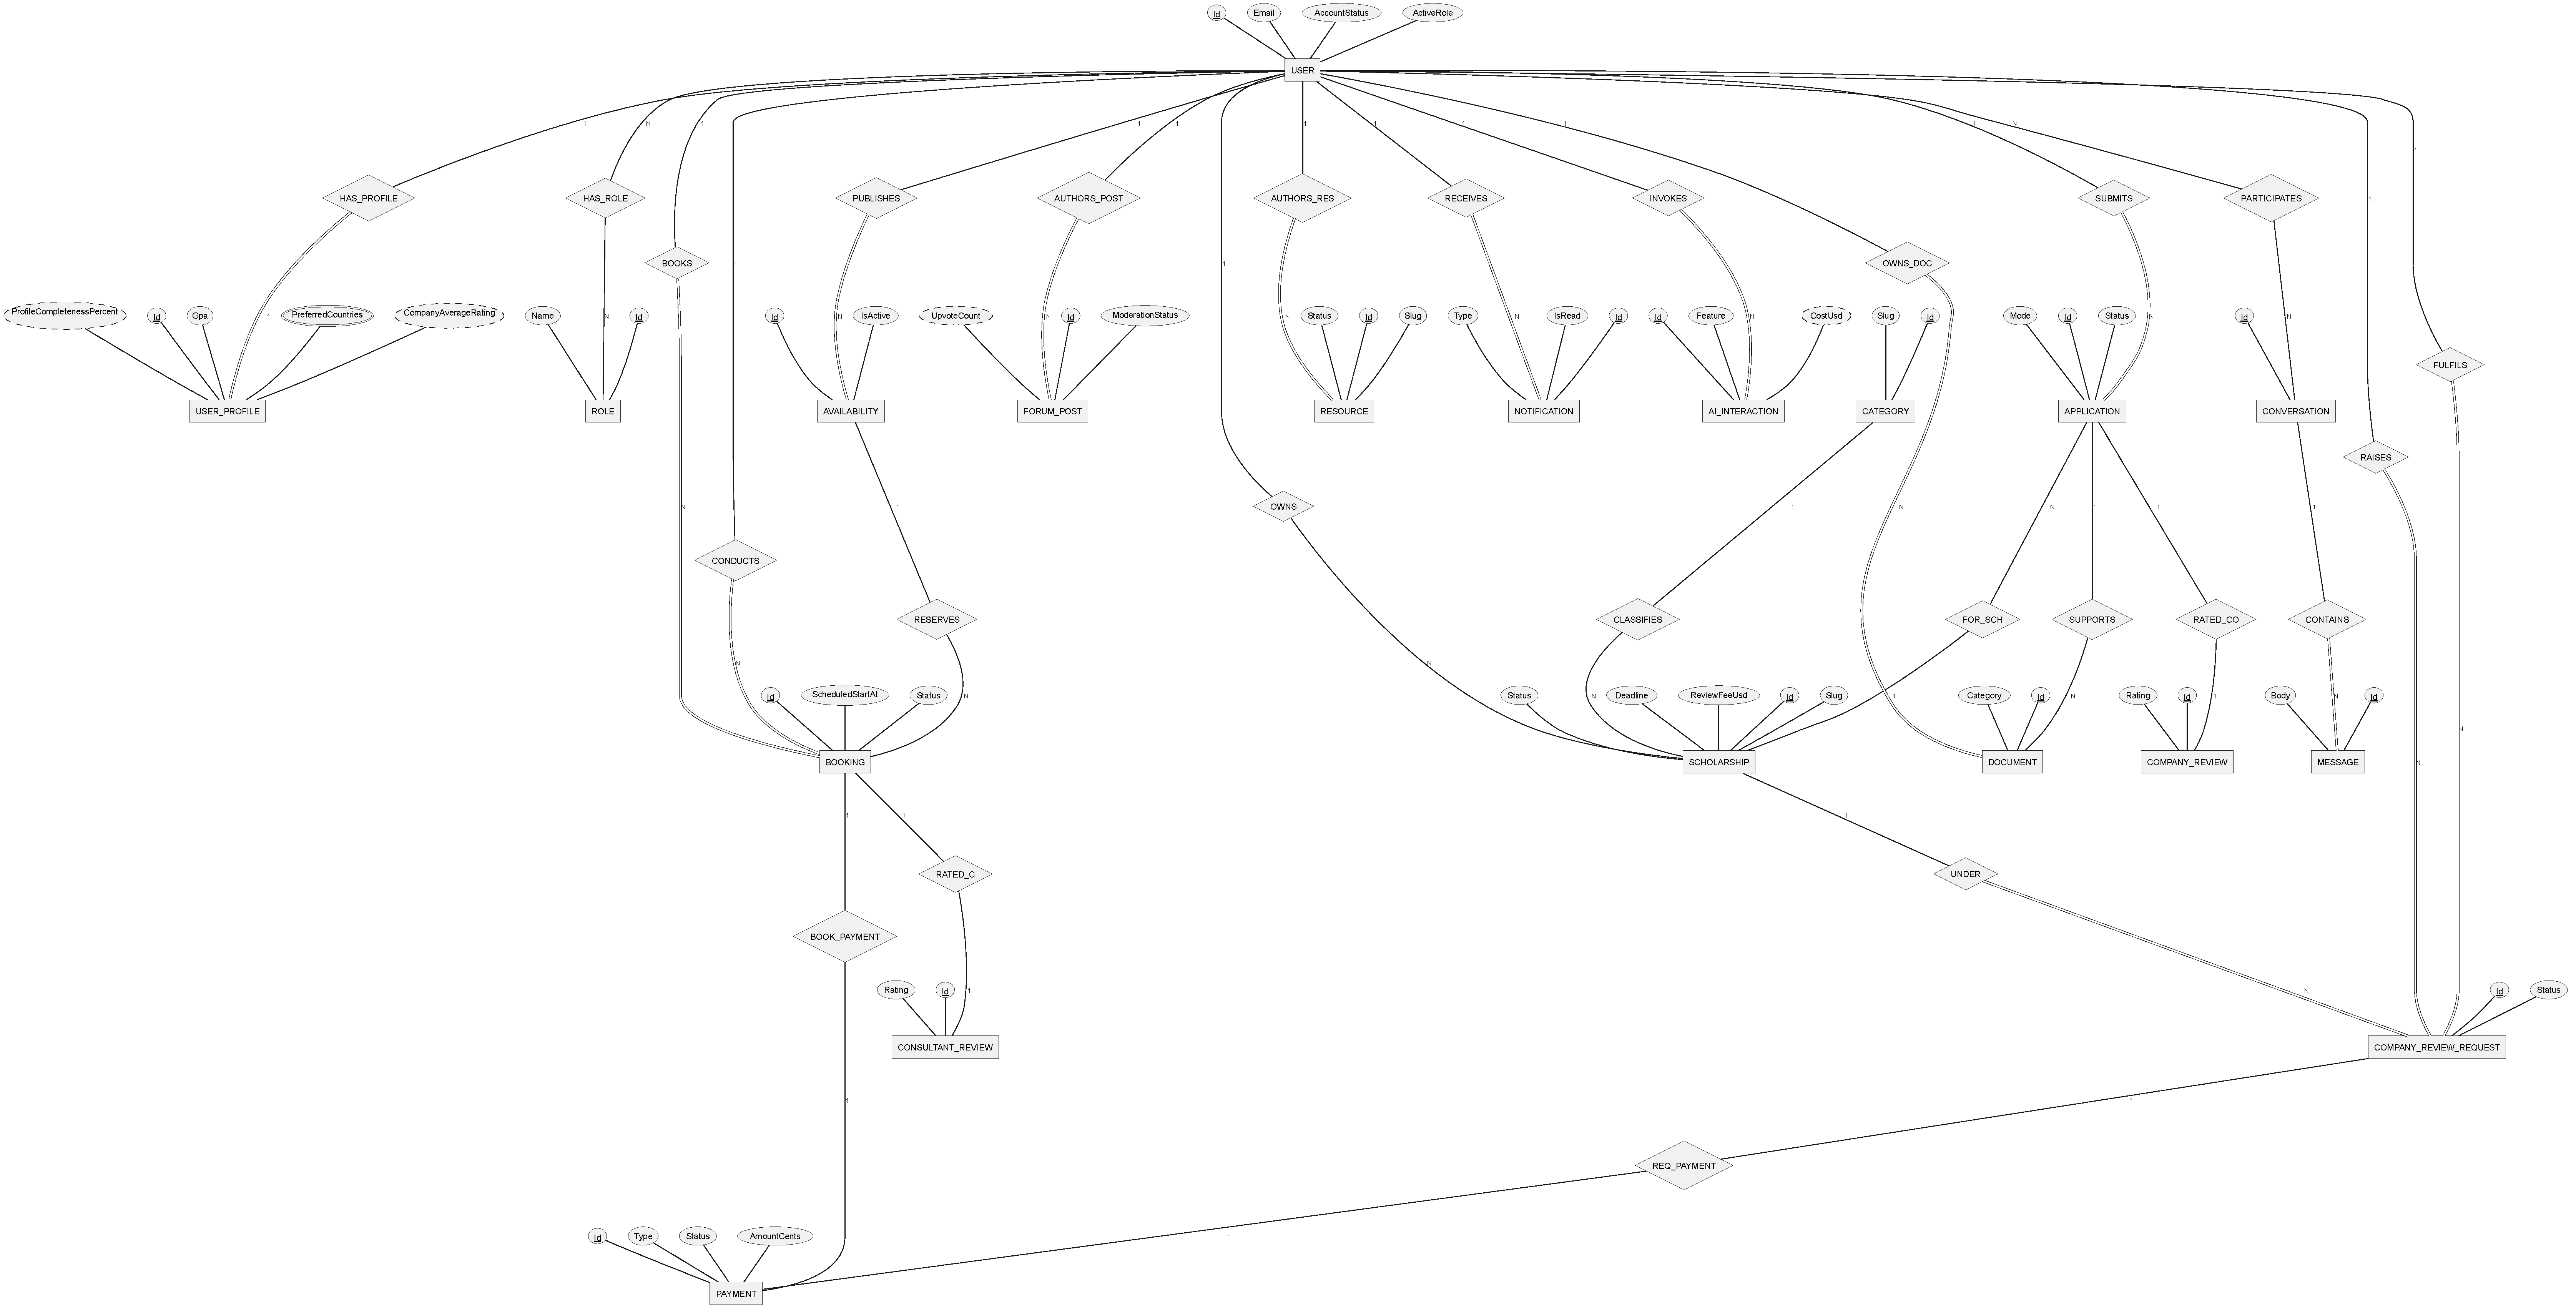
\includegraphics[width=\linewidth,height=0.92\textheight,keepaspectratio]{ScholarPath_EERD_Core.pdf}
\caption{Consolidated conceptual EERD (Chen notation).}
\end{figure}
\end{landscape}

\end{document}
